\documentclass[a4paper,12pt,russian]{extreport}
\usepackage[utf8]{inputenc}
\usepackage[T2A]{fontenc}
\usepackage[russian]{babel}
\usepackage{graphicx}
\usepackage{amsmath}

% далее две строки отвечающие за т.н. "полуторный интервал"
%\usepackage[nodisplayskipstretch]{setspace}
%\onehalfspacing
%\parskip 1.5ex % paragraph spacing

\usepackage{geometry}
\geometry{left=3cm}
\geometry{right=1.5cm}
\geometry{top=2cm}
\geometry{bottom=2cm}

%\renewcommand{\rmdefault}{ftm} 
%\frenchspacing

\usepackage{authblk}
\title{Отчет по лабораторной работе №3 «Решение СЛАУ прямыми методами. Теория возмущений» Вариант~№22}
\author{Левицкий Валентин А-13-22}
\affil{НИУ «МЭИ»}
\date{\today}
\begin{document}

\maketitle
\section*{Задача 2.1}
Методом простой итерации найти вещественные корни нелинейного уравнения $f(x)=0$ с точностью $\varepsilon = 10^{-8}$.

\[ f(x) = x^3 - 0.9x^2 - x - 0.1. \]

\subsection*{Решение}
Построим график функции и определим отрезки локализации для каждого корня:

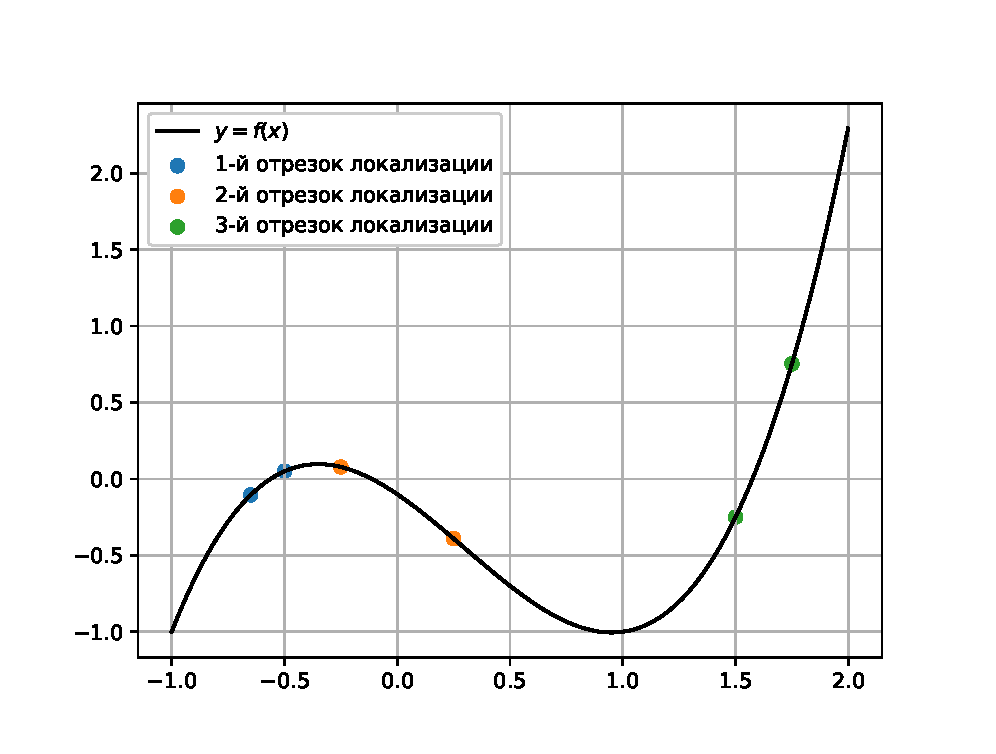
\includegraphics[width=\textwidth]{211.eps}

Определим производную $f(x)$:
\[ f'(x) = 3x^2 - 1.8 x - 1. \]
Построим график производной и отметим на нём границы отрезков локализации:

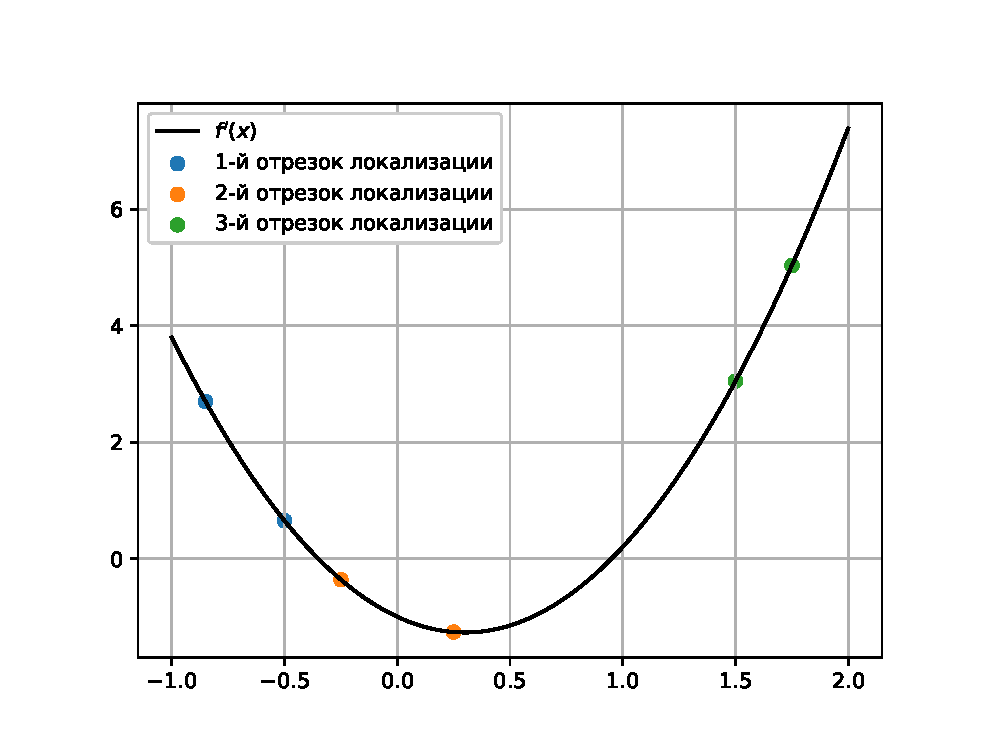
\includegraphics[width=\textwidth]{212.eps}

Из графика видно, что на отрезках локализации производная функции сохраняет постоянный знак.

Для каждого корня определим итерационный параметр $\alpha$ и параметр $q$, используя формулы:
\[ \alpha = \frac{2}{M1 + m1}, \]
\[ q = \left| \frac{M1 - m1}{M1 + m1} \right|, \]
где $M1=\max\limits_{x\in [a,b]} f'(x),\ m1 = \min\limits_{x\in [a,b]}f'(x)$.

Составим программу для нахождения корня с заданной точностью $\varepsilon$ по методу простых итераций. В качестве расчетной формулы используем метод простой итерации с параметром:
\[ x_{n + 1} = x_n - \alpha f(x_n). \]

\begin{verbatim}
def MPI(x0, M1, m1, f, eps):
    alpha = 2 / (M1 + m1)
    q = np.abs((M1 - m1) / (M1 + m1))
    x1 = x0 - alpha * f(x0)
    it = 1
    while abs(x1 - x0) > (1 - q) * eps / q:
        x0, x1 = x1, x1 - alpha * f(x1)
        it += 1
    print(f"Выполнено {it} итераций, x = {x1}")
    return x1
\end{verbatim}

Запишем результаты вычислений в таблицу:

{
\centering
\bgroup
\def\arraystretch{1.5}%
\begin{tabular}{|cccccc|c|}
\hline
\multicolumn{6}{|l|}{Левицкий Валентин Димитриевич A-13-22}                        & Вариант №22            \\ \hline
\multicolumn{6}{|l|}{\( f(x) = x^3 - 0.9x^2 - x - 0.1 \)}                        & \multicolumn{1}{c|}{ \( \varepsilon=10^{-8} \)}  \\ \hline
    \multicolumn{1}{|c|}{Корни}               & \multicolumn{1}{c|}{ \( [a,b] \)}                & \multicolumn{1}{c|}{ \( M_1 \)}          & \multicolumn{1}{c|}{ \( m_1 \)} & \multicolumn{1}{c|}{ \( \alpha \)}   & \multicolumn{1}{c|}{ \( q \)}             & \multicolumn{1}{c|}{Итерации}  \\ \hline
\multicolumn{1}{|c|}{$x_1 = -0.56224597$} & \multicolumn{1}{c|}{$[-0.65, -0.5]$} & \multicolumn{1}{c|}{$1.4375$}  & \multicolumn{1}{c|}{$0.65$}    & \multicolumn{1}{c|}{$0.9581$}  & \multicolumn{1}{c|}{$0.3772$} & \multicolumn{1}{c|}{8} \\
\multicolumn{1}{|c|}{$x_2 = -0.11291429$} & \multicolumn{1}{c|}{$[-0.25, 0.25]$} & \multicolumn{1}{c|}{$-0.3625$} & \multicolumn{1}{c|}{$-1.2625$} & \multicolumn{1}{c|}{$-1.2308$} & \multicolumn{1}{c|}{$0.5538$} & \multicolumn{1}{c|}{8} \\
\multicolumn{1}{|c|}{$x_3= 1.57516025$}   & \multicolumn{1}{c|}{$[1.5, 1.75]$}   & \multicolumn{1}{c|}{$5.0375$}  & \multicolumn{1}{c|}{$3.05$}    & \multicolumn{1}{c|}{$-0.1129$} & \multicolumn{1}{c|}{$1.5752$} & \multicolumn{1}{c|}{8} \\ \hline
\end{tabular}
\egroup
}

\section*{Задача 2.2}
Дано уравнение $f(x) = 0$. Найти все корни уравнения с заданной точностью $\varepsilon = 10^{-12}$ на указанном отрезке $[a, b]$. Для решения задачи использовать метод Ньютона и метод простых итераций. Сравнить количество итераций, потребовавшихся для достижения заданной точности каждым методом.
\[f(x) = 10^{-\sqrt{x}}- \sin(\pi \sqrt{x})- 0.9,\]
\[x \in [0, 3].\]

\subsection*{Решение}
Найдем отрезки локализации для каждого корня и середины этих отрезков примим за начальные приближения.

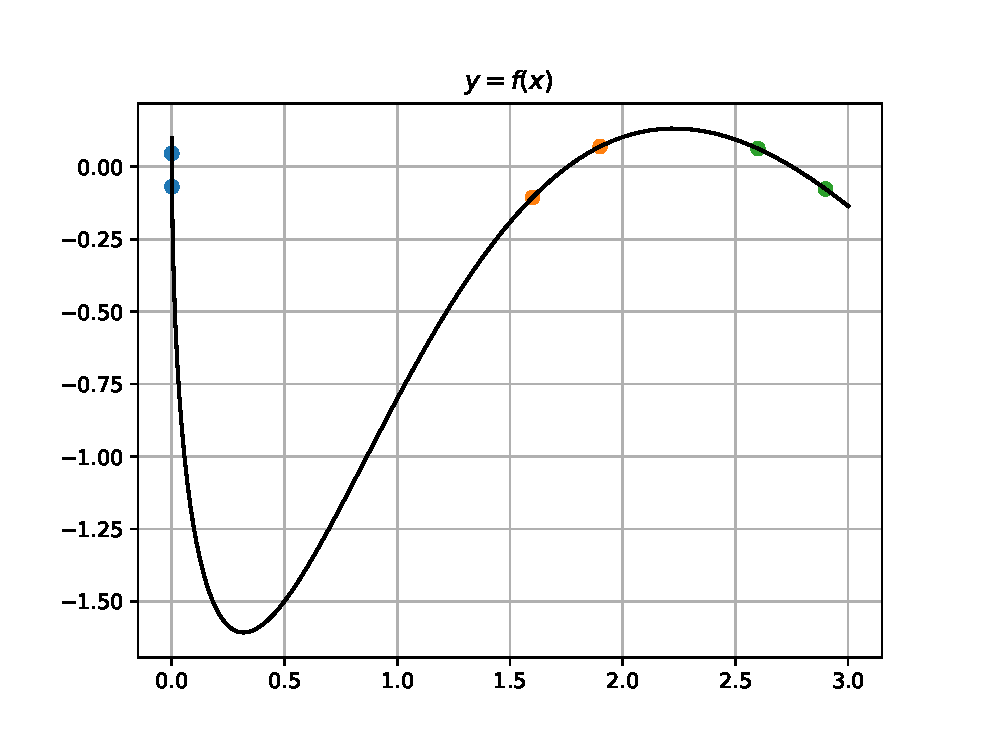
\includegraphics[width=\textwidth]{221.eps}

Составим программу вычисления корня методом Ньютона, предусмотрев в ней подсчёт числа итераций. Найдем с заданной точностью корни уравнения на отрезке $[0, 3]$.

\begin{verbatim}
def newton(x0, func, dfunc, eps):
    x1 = x0 - func(x0) / dfunc(x0)
    it = 1
    while abs(x1 - x0) > eps:
        x0 = x1
        x1 = x0 - func(x0) / dfunc(x0)
        # print(f"\t{x1}")
        it += 1
    print(f"\tВыполнено {it} итераций. x = {x1}")
    return x1
\end{verbatim}

Результаты для каждого из отрезков локализации:
\begin{verbatim}
Выполнено 5 итераций. x = 0.000343705625
Выполнено 4 итераций. x = 1.755702317447
Выполнено 4 итераций. x = 2.751734381135
\end{verbatim}

Составим программу вычисления корня методом простых итераций, предусмотрев в ней подсчёт числа итераций. Найдем с заданной точностью те же корни уравнения.
\begin{verbatim}
def MPI(x0, m1, M1, f, eps):
    alpha = 2 / (m1 + M1)
    q = abs((M1-m1)/ (M1 + m1))
    x1 = x0 - alpha * f(x0)
    it = 1
    while abs(x1 - x0) > (1 - q) * eps / q:
        x0 = x1
        x1 = x0 - alpha * f(x0)
        it += 1
    print(f"\tВыполнено {it} итераций. x = {x1}")
    return x1
\end{verbatim}
Результаты для каждого из отрезков локализации:
\begin{verbatim}
Выполнено 13 итераций. x = 0.000343705625
Выполнено 7 итераций. x = 1.755702317447
Выполнено 7 итераций. x = 2.751734381135
\end{verbatim}

Полученные результаты запишем в таблицу:

{
\centering
\bgroup
\def\arraystretch{1.5}%
\begin{tabular}{|llll|}
\hline
\multicolumn{4}{|l|}{$f(x) = 10^{-\sqrt{x}}- \sin(\pi \sqrt{x})- 0.9$}                                                                                                                                                                                              \\ \hline
\multicolumn{4}{|l|}{Расчетная формула метода Ньютона: $x_{n+1} = x_n - \dfrac{f(x_n)}{f'(x_n)}$}                                                                                                                                                                   \\ \hline
\multicolumn{4}{|l|}{Расчетная формула метода простых итераций: $x_{n+1} = x_n - \alpha f(x_n)$}                                                                                                                                                                    \\ \hline
\multicolumn{4}{|l|}{Задача 2.2}                                                                                                                                                                                                                                    \\ \hline
\multicolumn{1}{|l|}{Начальное приближение} & \multicolumn{1}{l|}{Корень уравнения} & \multicolumn{1}{l|}{\begin{tabular}[c]{@{}l@{}}Число итераций\\ Метод Ньютона\end{tabular}} & \begin{tabular}[c]{@{}l@{}}Число итераций\\ Метод простых итераций\end{tabular} \\ \hline
\multicolumn{1}{|l|}{0.00055}               & \multicolumn{1}{l|}{0.00034370562}    & \multicolumn{1}{l|}{5}                                                                      & 13                                                                              \\ \hline
\multicolumn{1}{|l|}{1.75}                  & \multicolumn{1}{l|}{1.755702317447}   & \multicolumn{1}{l|}{4}                                                                      & 7                                                                               \\ \hline
\multicolumn{1}{|l|}{2.75}                  & \multicolumn{1}{l|}{2.751734381135}   & \multicolumn{1}{l|}{4}                                                                      & 7                                                                               \\ \hline
\end{tabular}
\egroup
}

Модифицируем методы так, чтобы каждый метод делал заданное количество итераций и на каждом шаге сохранял значение модуля невязки $r_n = |f(x_n)|$.
\begin{verbatim}
def newton2(x0, func, dfunc, n, eps):
    x1 = x0 - func(x0) / dfunc(x0)
    r = [abs(f(x1))]
    it = 1
    while it < n:
        x0 = x1
        x1 = x0 - func(x0) / dfunc(x0)
        r.append(abs(f(x1)))
        it += 1
    return x1, np.array(r)

def MPI2(x0, m1, M1, f, n, eps):
    alpha = 2 / (m1 + M1)
    q = abs((M1-m1)/ (M1 + m1))
    x1 = x0 - alpha * f(x0)
    r = [abs(f(x1))]
    it = 1
    while it < n:
        x0 = x1
        x1 = x0 - alpha * f(x0)
        r.append(abs(f(x1)))
        it += 1
    return x1, np.array(r)
\end{verbatim}

Для каждого начального приближения вызовем модифицированные методы так, чтобы они проделали 10 итераций. Построим графики зависимости $r_n$ от $n$ в логарифмической шкале.

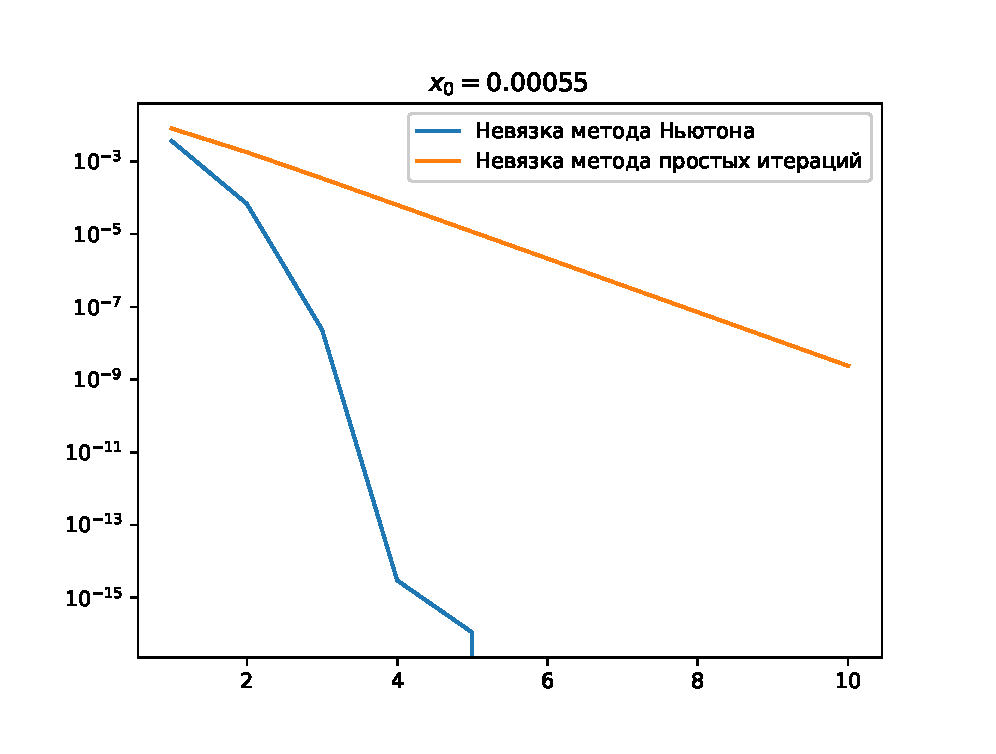
\includegraphics[width=12cm]{222_0.eps}

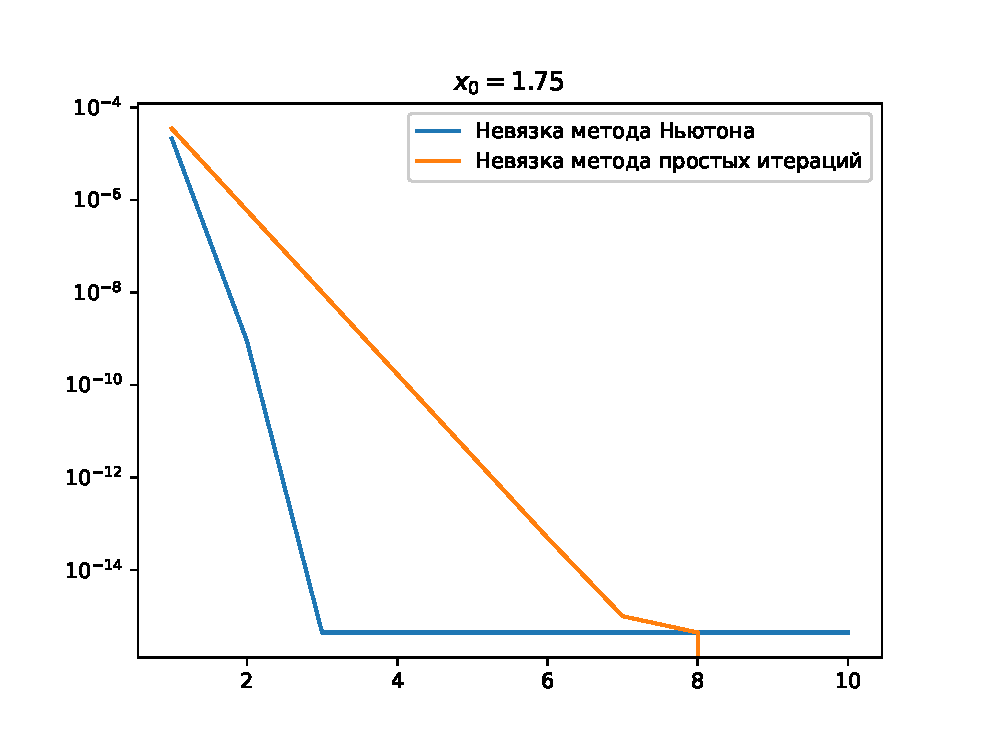
\includegraphics[width=12cm]{222_1.eps}

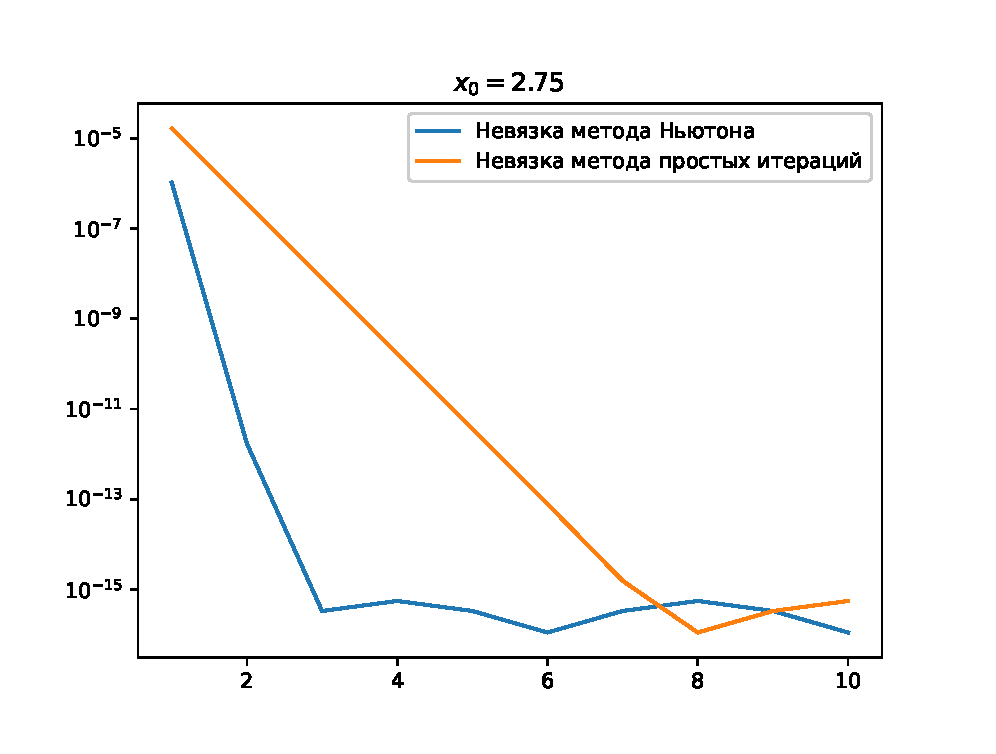
\includegraphics[width=12cm]{222_2.eps}

По полученым графикам можно сделать следующий вывод:

1. Возможно приблизительно определить порядок сходимости методов: для метода Ньютона он равен 2, для метода простых итераций $~1.6$.

2. Больший порядок сходимости позволяет методу быстрее приближаться к точному значению корня, что соответствует теоретическим результатам.

3. Невязка не будет стремиться к нулю из-за погрешности округления значений в памяти компьютера, а также из-за наличия интервала неопределенности корня.

4. Возможно, что начиная с какой-то итерации невязка будет равна нулю (1 график), если компьютер позволяет сохранить точное значение данного корня в памяти.

\section*{Задача 3.3}
Дана система уравнений $Ax = b$ c матрицей $A$ из задачи 3.2 и вектором $b:\ b_i = |N - 25| + 5$, где N - номер варианта. Решить систему методом Якоби с точностью $\varepsilon = 10^{-10}$.

\subsection*{Решение}
1. Составим программу преобразования системы $Ax = b$ к виду $x = Bx + c$.

\begin{verbatim}
def Jacobi(A, b):
    '''Перобразует СЛАУ Ax=b к виду x = Bx + c.'''
    B = np.zeros_like(A)
    c = np.zeros_like(b)
    for i in range(A.shape[1]):
        B[i, :] = -A[i, :] / A[i, i]
        B[i, i] = 0
        c[i,0] = b[i,0] / A[i, i]
    return B, c
\end{verbatim}

Убедимся, что выполнено достаточное условие сходимости метода: $||B|| < 1$
\begin{verbatim}
B, c = Jacobi(A, b)
np.linalg.norm(B)

0.6428766787355629
\end{verbatim}

2. Составим программу метода простых итераций с подсчетом нормы вектора невязки на каждой итерации.
\begin{verbatim}
def MPI(A, b, eps):
    B, c = Jacobi(A, b)
    x0 = c
    x1 = B.dot(x0) + c
    iters = 1
    r_n = []
    k = (1 - inf_norm(B)) / inf_norm(B)
    while inf_norm(x1 - x0) > k * eps:
        r_n.append(euclid_norm(A.dot(x1) - b))
        x0 = x1
        x1 = B.dot(x1) + c
        iters +=1
    print("Выполнено итераций: ", iters)
    return x1, np.array(r_n)
\end{verbatim}

Убедимся, что выполнено достаточное условие сходимости метода: $||B|| < 1$.
\begin{verbatim}
B, c = Jacobi(A, b)
np.linalg.norm(B)

0.6428766787355629
\end{verbatim}

Составим программу метода простых итераций с подсчетом нормы вектора невязки на каждой итерации.
\begin{verbatim}
def MPI(A, b, eps):
    B, c = Jacobi(A, b)
    x0 = c
    x1 = B.dot(x0) + c
    iters = 1
    r_n = []
    k = (1 - inf_norm(B)) / inf_norm(B)
    while inf_norm(x1 - x0) > k * eps:
        r_n.append(euclid_norm(A.dot(x1) - b))
        x0 = x1
        x1 = B.dot(x1) + c
        iters +=1
    print("Выполнено итераций: ", iters)
    return x1, np.array(r_n)
\end{verbatim}

Найдем решение задачи с заданной точностью.

\begin{verbatim}
x, r_n = MPI(A, b, eps)

Выполнено итераций:  13
\end{verbatim}

Подставим найденое решение в исходное уравнение и убедимся в корректности метода:
\begin{verbatim}
A.dot(x).T

array([[8., 8., 8., 8., 8., 8., 8., 8., 8., 8., 8., 8., 8., 8., 8., 8.,
        8., 8., 8., 8.]])
\end{verbatim}

Нормы векторов невязки по итерациям:

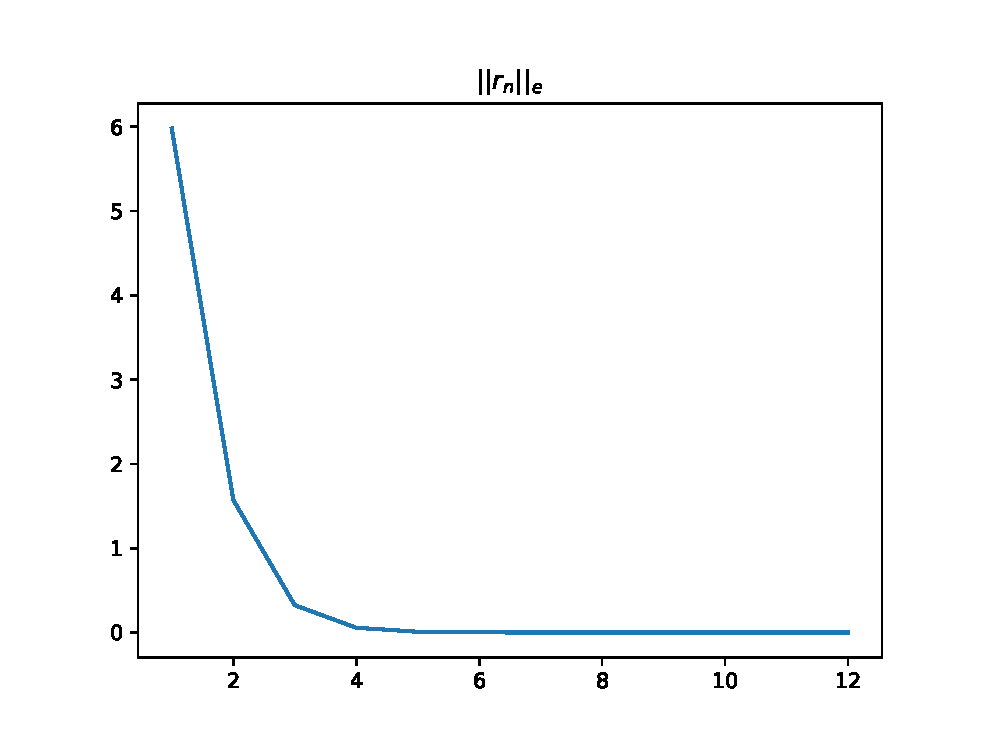
\includegraphics[width=15cm]{fig331.eps}

\end{document}
